\documentclass[10pt,sans,english,compress,xcolor=dvipsnames]{beamer}
\author[Lily ]{ Dr Lily Asquith (Lily, she/her)}

\usetheme{Szeged}
%\defbeamertemplateparent{enumerate items}{enumerate item,enumerate subitem,enumerate subsubitem,enumerate mini template}
\definecolor{titcol}{RGB}{16,78,100} 
\setbeamercolor{frametitle}{fg=titcol,bg=White}
\useoutertheme{miniframes} 
\useinnertheme{rectangles}

\usepackage{pifont}
\newcommand{\tick}{\textcolor{grn}{\ding{52} } }
\newcommand{\nope}{\textcolor{red}{\ding{54} } }


\usepackage{soul}
\usepackage{cancel}

\usepackage[most]{tcolorbox}
\definecolor{LilyBlack}{rgb}{0.05,0.1,0.3} % UBC Blue (primary)
\usecolortheme[named=LilyBlack]{structure}

\usepackage{booktabs}
\usepackage{tabularx}
%\usepackage{tikz}
%\def\checkmark{\tikz\fill[scale=0.4](0,.35) -- (.25,0) -- (1,.7) -- (.25,.15) -- cycle;}

\usepackage{physics}

\usepackage{xparse}

\setbeamertemplate{footline}{%
  \leavevmode%
  \hbox{\begin{beamercolorbox}[wd=.5\paperwidth,ht=2.5ex,dp=1.125ex,leftskip=.3cm plus1fill,rightskip=.3cm]{author in head/foot}%
    \usebeamerfont{author in head/foot}\insertshortauthor
  \end{beamercolorbox}%
  \begin{beamercolorbox}[wd=.5\paperwidth,ht=2.5ex,dp=1.125ex,leftskip=.3cm,rightskip=.3cm plus1fil]{title in head/foot}%
    \usebeamerfont{title in head/foot}\insertshorttitle\hfill\insertframenumber\,/\,\inserttotalframenumber
  \end{beamercolorbox}}%
  \vskip0pt%
}

\DeclareMathSizes{10}{10}{6}{4} % this one
%\DeclareMathSizes{10.95}{10}{6}{4}   % For size 10 text

\newcommand*\ColorBox[3][black]{%
  \makebox[2em][c]{%
    \setlength\fboxsep{-.5\fboxrule}%
    \raisebox{\dimexpr-#3em+.5ex}{%
      \fcolorbox{#1}{#2}{%
        \rule{0pt}{\dimexpr#3em*2}%
        \rule{\dimexpr#3em*2}{0pt}%
      }%
    }%
  }%
}

\usepackage{hyperref}
\hypersetup{
    colorlinks=true,
    linkcolor=blue,
    filecolor=magenta,      
    urlcolor=blue,
    pdftitle={Overleaf Example},
    pdfpagemode=FullScreen,
    }

\urlstyle{same}

% this part excludes specified frames from counters in navigation bar
\makeatletter
\let\beamer@writeslidentry@miniframeson=\beamer@writeslidentry
\def\beamer@writeslidentry@miniframesoff{%
  \expandafter\beamer@ifempty\expandafter{\beamer@framestartpage}{}% does not happen normally
  {%else
    % removed \addtocontents commands
    \clearpage\beamer@notesactions%
  }
}
\newcommand*{\miniframeson}{\let\beamer@writeslidentry=\beamer@writeslidentry@miniframeson}
\newcommand*{\miniframesoff}{\let\beamer@writeslidentry=\beamer@writeslidentry@miniframesoff}
\makeatother


\makeatletter
\newcommand\notsotiny{\@setfontsize\notsotiny{6.5}{7.5}}
\makeatother




\usepackage{multicol}
\usepackage{sansmath}
\usepackage{minted}
\definecolor{LightGray}{gray}{0.95}
\usepackage{nicematrix}

\title[Uncertainties]{Correlations \& Uncertainties}
\date{}
\titlegraphic{
%\center

\includegraphics[scale=0.15]{sussex-logo}
}
% Lily includes for font and spacing
\usepackage{cmbright} % pretty nice but maybe a bit too different
\renewcommand{\baselinestretch}{1.1} 
\usepackage{sansmath}


\begin{document}

\newcommand\info{\mathcal{J}_{\theta}}
\newcommand\loglike{\ln{ \mathcal{L}_{\theta}} }
\newcommand\like{\mathcal{L}_{\theta} }

\newcommand\thetahat{\hat{ \theta }  }

\definecolor{grn}{RGB}{0,128,0} 
\newcommand{\gbl}[1]{\textcolor{grn}{#1}}

\definecolor{wh}{rgb}{0.95, 0.95, 0.96}
\newcommand{\wht}[1]{\textcolor{wh}{#1}}

%\newcommand{\inprob}{\overset{p}{\to}}

\newcommand{\boo}[1]{\textbf{\textcolor{red}{#1}}}

\newcommand{\covmat}{\mathbf{\textcolor{magenta}{\Sigma}} }


\definecolor{purr}{RGB}{128,0,128} 
\newcommand{\purp}[1]{\textcolor{purr}{#1}}

\newcommand{\magt}[1]{\textbf{\textcolor{magenta}{#1}}}
 \newcommand{\magtn}[1]{\textcolor{magenta}{#1}}
 
%\definecolor{bbl}{RGB}{128,0,128} 
\newcommand{\bbl}[1]{\textcolor{blue}{#1}}

\newcommand{\rbl}[1]{\textcolor{red}{#1}}

\definecolor{dblu}{RGB}{37,150,190} 
\newcommand{\blu}[1]{\textcolor{dblu}{#1} }

\definecolor{dor}{RGB}{255,40,0} 
\newcommand{\dor}[1]{\textcolor{dor}{#1} }

\definecolor{darkgreen}{RGB}{46,139,87} 
\newcommand{\dgreen}[1]{\textbf{\textcolor{darkgreen}{#1}} }
%\newcommand{\gbl}[1]{\textcolor{darkgreen}{#1}}

\definecolor{lgray}{RGB}{222,222,222} 

\definecolor{lyellow}{RGB}{255,255,224} 

\newcommand{\E}[1]{\mathbf{E}_{#1}}
%
\newcommand{\rvX}[1]{X_{(#1)} } 

\newcommand{\rvY}[1]{Y_{(#1)} }

\newcommand{\rvx}[1]{x_{(#1)} } 

\newcommand{\rvy}[1]{y_{(#1)} }



\newcommand{\red}[1]{\textcolor{red}{#1} }

\newcommand{\bluedots}{\blu{\ldots} }

\newcommand{\dordots}{\dor{\ldots} }


\newcommand{\where}{\dgreen{\;where\;} }


\newcommand{\pand}{\dgreen{\;and\;} }
\newcommand{\por}{\dgreen{\;or\;} }

\newcommand{\sumN}{ \sum\limits_{\blu{i}}^{\blu{N}} }

\newcommand{\sumZ}{ \sum\limits_{\dor{j}}^{\dor{Z}} }

\newcommand{\Expec}[1]{ \mathbb{E}[#1] }


\newcommand{\Xfj}[1]{ X_{ \dor{#1} } }

\newcommand{\xfi}[1]{ x_{ \blu{#1} } }

\newcommand{\Xij}[2]{ X_{\mage{#1},\blu{#2} }}

\newcommand{\sumxi}{ \sumN \xfi{i} }

\newcommand{\sumXj}{ \sumZ \Xfj{j} }

\newcommand{\sumZa}[1]{ \sumZ {#1}_{ \dor{j} } }

\newcommand{\sumZab}[2]{ \sumZ {#1}_{ \dor{j} }\, {#2}_{ \dor{j} } }

\newcommand{\sumNab}[2]{ \sumN {#1}_{ \blu{i} }\, {#2}_{ \blu{i} } }

\newcommand{\vecxi }{ [ \xfi{1} \xfi{2}, \bluedots, \xfi{N} ] }

\newcommand{\vecXj }{ [ \Xfj{1} \Xfj{2}, \bluedots, \Xfj{Z} ] }

\newcommand{\vecXij }{ [ \Xij{1}{1} \Xij{1}{2}, \bluedots, \Xij{1}{N_1} ],\, [ \Xij{2}{1} \Xij{2}{2}, \bluedots, \Xij{2}{N_2} ],\, \dordots,\,[ \Xij{Z}{1} \Xij{Z}{2}, \bluedots, \Xij{Z}{N_Z} ] }

% definitions

\newcommand{\overNblack}{ \dfrac{1}{N} }
\newcommand{\overN}{ \dfrac{1}{ \blu{N} } }

\newcommand{\defmean }{ \overline{x} = \overN \sumN \xfi{i} }

\newcommand{\meanx }{ \overline{x} }
\newcommand{\meansqx }{ \overline{x^2} }
\newcommand{\sqmeanx }{ \overline{x}^2 }
\newcommand{\devsq}{ (\xfi{i} - \meanx)^2 }

%\newcommand{\var }[1]{ \mathcal{V}_{#1} }
\newcommand{\defvar }{ \var{x} = \overN \sumN \devsq }
\newcommand{\defvarshort }{ \var{x} = \meansqx - \sqmeanx }

\newcommand{\defstd }{ s_x = \sqrt{ \var{x} }  }

\newcommand{\defwmean }{ \overline{X} = \dfrac{ \sumZab{w}{X} }{ \sumZa{w} } }  

\newcommand{\defw }{ w_{\dor{j}} = \dfrac{1}{ \var{\Xfj{j} } } }



\begin{frame}
\titlepage
\end{frame} 

%\section*{Preamble}
\begin{frame}

\begin{center}
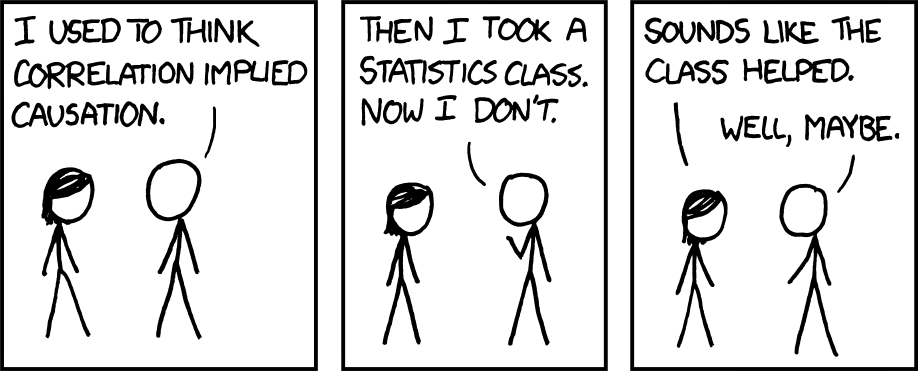
\includegraphics[scale=0.7]{xkcd-correl}

\small
\href{https://xkcd.com/552/}{https://xkcd.com/552/}
\end{center}

\end{frame} 



% contents
\begin{frame}{Correlations \& Uncertainties}
\large
\begin{itemize}
\item Variance, again\\[1ex]
\item Covariance Matrix \\[1ex]
\item Linear Correlations \& Independence \\[1ex]
%\item Principal Components \\[1ex]
\item Uncertainty Propagation:  linear functions \\[1ex]
\item Taylor Series approach \\[1ex]
\item Uncertainty Propagation:  nonlinear functions \\[1ex]
\end{itemize}

\end{frame} 


\begin{frame}{Intro, reminder of big picture}

\footnotesize
I mentioned in our first lecture that \textbf{measurements are meaningless without quoted uncertainties}. \\[1ex]
There are two classes of uncertainty:
\begin{enumerate}
\item \textbf{Systematic}: My scale is not calibrated; a train from Geneva to Paris is causing a skew in my measurements; ...\\
\item \textbf{Statistical}: I don't have enough data (wish I had $N\rightarrow \infty$!) OR I have loads of data, but it has intrinsic \textbf{Variance}.\\
\end{enumerate}

\blu{We aren't thinking about systematics at all in this module, which is nice for me as I think about nothing but systematics in my day job.}\\
\textbf{Very often, the thing we want to measure is not directly obtainable. It is a function of the RVs we measure, rather than the RVs themselves. \boo{How do we propagate the statistical uncertainties from the RVs to the function?} }\\[1ex]
%\footnotesize
%\blu{This week's material is very mathy. We need math to convince ourselves that we can do this very important job the right way.}

\end{frame} 




\section{Variance}

\begin{frame}{Variance Recaps}
\footnotesize

We know how to write down the (unbiased) variance for a set of measurements of a single RV, $K$:\\[1ex]

$V[K] = \dor{\dfrac{1}{(N-1)}}\sum\limits_i^N \purp{(k_i - \overline{k})^2} $ \blu{ }\\[2ex]

\begin{itemize}
\item The term $\purp{(k_i - \overline{k})^2}$ is the variance of the $i^{th}$ measurement, $k_i$.
\item The sum is over the $N$ measurements.
\item We are not far from being ready to show that we need \dor{$N-1$} in the denominator rather than \dor{$N$}.
\end{itemize}

\end{frame} 


\begin{frame}{Pictorially}
\footnotesize

$V[K] =\dfrac{1}{(N-1)}\sum\limits_i^N$  \colorbox{lgray}{$(k_i - \overline{k})^2$}  \blu{ }\\[1ex]
We can't draw the \colorbox{lgray}{variance} on an axis with units of $k$. \\[1ex]
We can draw the \boo{standard deviation} \colorbox{lyellow}{$\sigma_k = \sqrt{V[k]}$}\\[1ex]

\centering
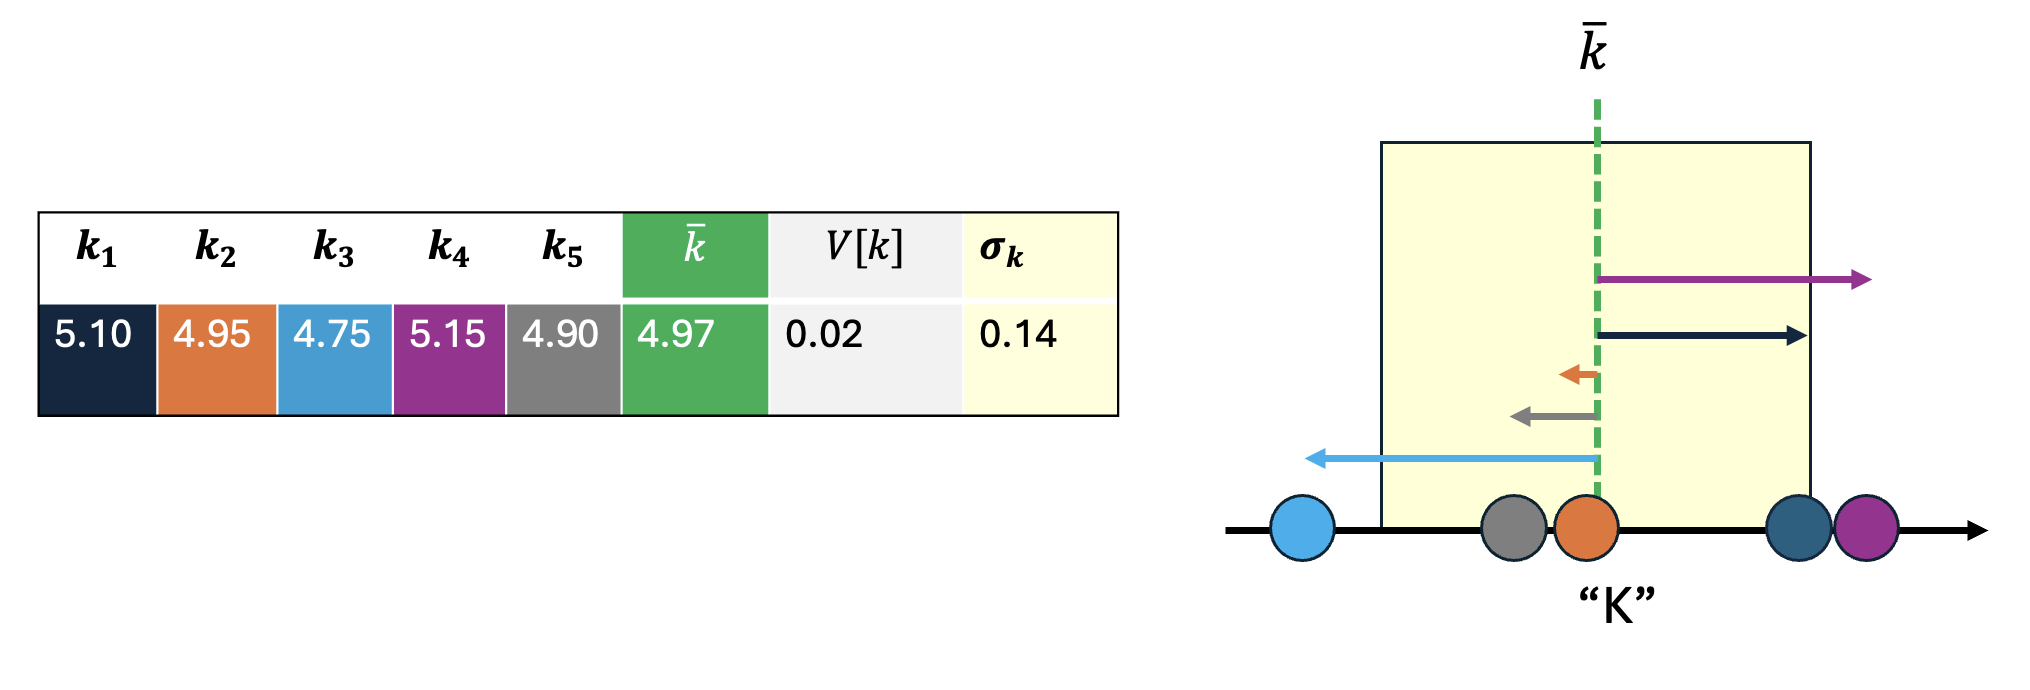
\includegraphics[scale=0.3]{recap1}

\end{frame} 


\begin{frame}{Pictorially}
\footnotesize

We can draw the \boo{standard deviation} \colorbox{lyellow}{$\sigma_k = \sqrt{V[k]}$}\\[1ex]

\centering
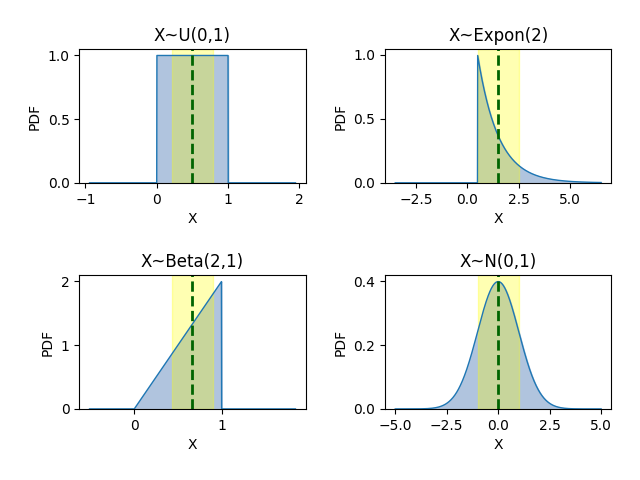
\includegraphics[scale=0.5]{MeanVarSigma}

\end{frame} 


\begin{frame}{Variance when we know the probability}
\footnotesize

$V[k] = \dor{\dfrac{1}{(N-1)}}\sum\limits_i^N \purp{(k_i - \overline{k})^2} $ \blu{ measurements are $k_i$}\\[2ex]

\textbf{If we know the probability of each measurement}, we can do away with the normalisation and write:\\[1ex]

$V[k] = \sum\limits_i^N$ \purp{ $(k_i - \overline{k})^2$} \dor{$p_{k_i} $}\\[1ex]

\dor{$p_{k_i}$} is the probability of measurement $k_i$. Crucially, $\sum\limits_i^N$\dor{$p_{k_i} $}=1. \\[2ex]

\blu{An example where we know the \dor{$p_{k_i} $} might be the outcomes of tossing a coin.}
\end{frame} 





\begin{frame}{True Variance}
\footnotesize

In the limit of an infinite number of measurements, data often corresponds to some \boo{true underlying distribution}.\\[1ex]

 The underlying distribution may be a PMF (discrete RV) or a PDF (continuous RV).\\[1ex]

$V[K] = \sum\limits_{k \in S}$ \purp{ $(k - E[K])^2$} \dor{$p_{k} $} \blu{for discrete $K$, PMF is $p_{k}$}.\\[1ex]


$V[X] = \int\limits_{x \in S} \purp{ (x - E[X])^2}\, \dor{f_X}\, dx$  \blu{for continuous $X$, PDF is $f_X$ }\\[1ex]

Now we use the Expected Value $E[K]$ (the True Mean) rather than the mean of the measurements $\overline{k}$

\end{frame} 


\begin{frame}{True Variance}
\footnotesize

Here is the True variance for a continuous RV $X$:\\[1ex]

$V[X] = \int\limits_{x \in S} \purp{ (x - E[X])^2}\, \dor{f_X}\, dx$ \\[1ex]

\dor{$f_X$} is the PDF value \textbf{for measurement $x$}. Crucially, $\int\limits_{-\infty}^{\infty}$\dor{$f_X $}=1. \\[1ex]

Also crucially, \dor{$f_X=0$} for any exact value of $x$, but when we integrate the PDF we get a probability.

\begin{itemize}
\item When the PDF is on its own outside the integral, it is zero. But when it is inside the integral, it is not zero.
\item The integral over the support is equal to the integral over infinity, because outside the support all probabilities are zero.
\end{itemize}
\end{frame} 

%
%
%\begin{frame}{Useful formula for true variance}
%
%$V[X] = \int\limits_{x \in S} \purp{ (x - E[x])^2}\, \dor{f_X(x)}\, dx$  \blu{for continuous $X$: measurements are x}\\[1ex]
%
%$V[X] = E[X^2] - E^2[X] = E[ (X- \mu_X)^2] $ \blu{most useful form}\\[1ex]
%
%\blu{Remember $E[X] \equiv \mu_X$: use confusing mixed notation because it is easier to read... }\\
%
%Let's check that it makes sense to us that these are equivalent definitions of variance.
%
%\end{frame} 


\begin{frame}{Variance in terms of expectation}
\footnotesize

$V[X] = \int\limits_{x \in S} \purp{ (x - E[x])^2}\, \dor{f_X(x)}\, dx$  \blu{for continuous $X$: measurements are x}\\[1ex]

Recall the definition of the Expected Value:\\[1ex]

$E[X] = \int\limits_{x \in S} x\, \dor{f_X(x)}\, dx$\\[1ex]

Therefore, with $x \rightarrow (x -E[x])^2 $:\\[1ex]

$E[\purp{ (x - E[x])^2}] = \int\limits_{x \in S} \purp{ (x - E[x])^2}\, \dor{f_X(x)}\, dx = V[X]$\\[1ex]

$V[X] = E[ (x - E[x] )^2]$ is the variance of $X$, by definition.\\

%We will turn to the definition of the expected value of a RV:\\[1ex]
%
%$E[X] = \int\limits_{-\infty}^{\infty} x\, f_X(x) dx$\\[1ex]
%
%\bbl{$E[X^2] = \int\limits_{-\infty}^{\infty} x^2\, f_X(x) dx$}\\[1ex]
%
%\rbl{$E^2[X] = \left( \int\limits_{-\infty}^{\infty} x\, f_X(x) dx\right)^2$}\\[1ex]

\end{frame} 

\begin{frame}{A proof I promised a while ago}
\footnotesize

$V[X] = \bbl{E[} (X - E[X] )^2\bbl{]}$ is the variance of $X$, by definition.\\

\small
\begin{align*}
V[X] & = \bbl{E[\,} X^2 + E^2[X] - 2X\,E[X] \bbl{\,]}\\
	& = \bbl{E[\,} X^2\bbl{\,]} + \bbl{E[\,} E^2[X] \bbl{\,]}- \bbl{E[\,}2\purp{X}\,E[X] \bbl{\,]}\;\; \blu{because\; E[A+B] = E[A] + E[B]} \\
	& = E[ X^2] + E^2[X] - 2E[X]  \bbl{E[}\purp{X}\,\bbl{]}\;\; \blu{because\; E[E[A]] = E[A]}\\
	& = E[ X^2] + E^2[X]  - 2E^2[X]   \\	
	& = E[ X^2] - E^2[X]   \\
\end{align*}

\normalsize
Now we have our useful definition of variance: $V[X] = E[X^2] - E^2[X] $ and hopefully no room for confusion about how we got there.

\end{frame} 


%
%
%\begin{frame}{Shorthand notation}
%
%The deviation of an RV from the mean of its distribution, $X-E[X]$, comes up over and over again, let's use a shorthand:\\
%
%\boo{$e_i = X_{(i)} - E[X_{(i)}]$}\\[2ex]
%
%%The $\sigma_i$ is the \boo{Standard Deviation}, recall $\sigma_X^2 = V[X] $. Now we can write:\\[1ex]
%
%$V[X_{(i)}] = E[(X_{(i)} - E[X_{(i)}])^2] \rightarrow$ \boo{$V[X_{(i)}] = E[e_i^2]$}\\[2ex]
%
%%$\mathsf{cov}[X_{(i)}, X_{(j)}] = E[(X_{(i)} - \mu_{X_{(i)}}) (X_{(j)} - \mu_{X_{(j)}})] \rightarrow$  \boo{$\mathsf{cov}[X_{(i)}, X_{(j)}] = E[\sigma_i\,\sigma_j]$}\\[1ex]
%\end{frame} 


\section{Variance Algebra}

\begin{frame}{Variance of two RVs: Covariance}
\footnotesize
Let's use shorthand $\rbl{e_X = X - E[X]}$, so $V[X] = \bbl{E[\,} (\rbl{X - E[X]} )^2\bbl{\,]} = \bbl{E[\,}\rbl{e_x}^2\bbl{\,]}$

\begin{align*}
%& = \bbl{E[\, } \rbl{(}  X+Y - E[X] - E[Y] \rbl{)}^2\bbl{ \,] }  \[1ex]
	    %& = \bbl{E[\,}\rbl{(}\,[X-E[X]] + [Y - E[Y]]\,\rbl{)}^2\bbl{\,]} \\[1ex]
V[X+Y]  & = \bbl{E[\,}(\rbl{e_x + e_y})^2\bbl{\,]} \hspace{10cm} \\[1ex]	    
            & = \bbl{E[\,} e_x^2 + e_y^2 +2 e_x e_y  \bbl{\,]} \\[1ex]
            & = \bbl{E[\,}  e^2_X\bbl{\,]} + \bbl{E[\,} e^2_Y\bbl{\,]} + 2\bbl{E[\,}  e_X  e_Y  \bbl{\,]} \\[1ex]
            & = V[X] + V[Y] + 2 \mathsf{cov}[X,Y]\\[1ex]
\end{align*}

\small
The expectation of the product of deviations is the \boo{Covariance}:\\

 $\bbl{E[\,}  e_X  e_Y  \bbl{\,]} = \bbl{E[\,}  (X-E[X])(Y-E[Y] ) \bbl{\,]} = \mathsf{cov}[X,Y]$\\[1ex]
 



 

\end{frame} 



\begin{frame}{Variance for \boo{independent} X,Y}
\footnotesize

Note that if (and only if) X and Y are independent: \\[1ex]

$\bbl{E[\,}  e_X  e_Y  \bbl{\,]}= \bbl{E[\,}  e_X\bbl{\,]} \bbl{E[\,}   e_Y  \bbl{\,]}$\\[1ex]

And  $E[e_x]=  E[X-E[X] ] = E[X]-E[X] = 0$\\[1ex]

For \boo{independent} RVs $X, Y $ we can write the variance of a sum as the sum of their variances:\\[1ex]

$V[X+Y] =  V[X] + V[Y]$\\[1ex]

\blu{The sum algebra is true for Expected values whether the RVs are independent or not: $E[X+Y] = E[X] + E[Y]$ always.}\\

\end{frame} 


\begin{frame}{Variance for \boo{dependent} X,Y}
\footnotesize

For \boo{dependent} RVs $X, Y $ we have an additional term in the variance of a sum:\\[1ex]

$V[X+Y] =  V[X] + V[Y] + 2\mathsf{cov}[X,Y]$\\[1ex]

This additional term is the \boo{Covariance}\\[1ex]

$\mathsf{cov}[X,Y] = E[ \sigma_X  \sigma_Y ]  = \bbl{E[\,}  (X-E[X])(Y-E[Y] ) \bbl{\,]} = E[XY] - E[X]E[Y]$\\[1ex]

\blu{The last form is analogous to  $V[X] = E[X^2] - E^2[X]$}.

\end{frame} 



\begin{frame}{Variance Algebra}
\small

Very useful: \boo{$V[aX] = a^2 V[X]$}\\[2ex]

\footnotesize
\begin{align*}
V[aX]   & = \bbl{E[\,} (aX -E[aX])^2\bbl{\,]} \hspace{10cm}\\[1ex]	    
            & = \bbl{E[\,} a^2X^2 + E^2[aX] - 2aXE[aX]  \bbl{\,]} \\[1ex]
            & = \bbl{E[\,} a^2X^2 + a^2E^2[X] - 2a^2XE[X]  \bbl{\,]} \\[1ex]
            & = a^2\bbl{E[\,} X^2\bbl{\,]} + a^2\bbl{E[\,} E^2[X]\bbl{\,]} - 2a^2E[X]\bbl{E[\,} X  \bbl{\,]} \\[1ex]
            & = a^2\left( \bbl{E[\,} X^2\bbl{\,]} + \bbl{E[\,} E^2[X]\bbl{\,]} - 2E^2[X]\right) \\[1ex]
            & = a^2 V[X] \\[1ex]            
\end{align*}

%Proof uses $V[X] = E[ (X- E[X] )^2 ]$\\[1ex]
%\vspace{5cm}



\end{frame} 


\begin{frame}{Covariance Algebra}
\small

\boo{Covariance of linear functions}:\\[1ex]
$\mathsf{cov}[\dgreen{$\alpha$}X + \purp{c}, \dgreen{$\beta$}Y + \purp{d}]= \dgreen{$\alpha\,\beta$}\,\mathsf{cov}[X,Y]$ for constants $\alpha$, $\beta$, c, d. \\[2ex]

\boo{Covariance with a sum}:\\[1ex]
$\mathsf{cov}[X+Y, Z] = \mathsf{cov}[X, Z ] + \mathsf{cov}[Y, Z ]$\\[1ex] 

\boo{Covariance with self}:\\[1ex]
$\mathsf{cov}[X, X]= V[X]$ \\[2ex]

\end{frame} 


\section{Covariance Matrix}

\begin{frame}
\centering
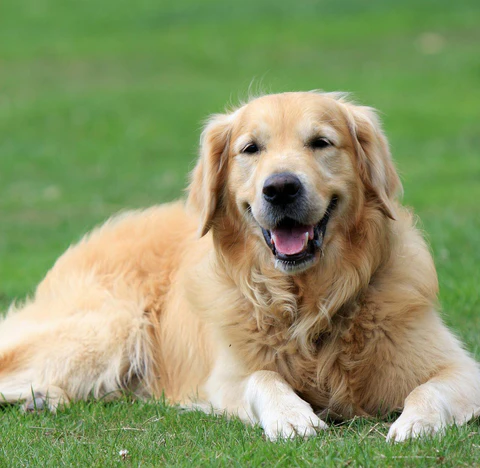
\includegraphics[scale=0.3]{doggo}
\end{frame}


\begin{frame}{Covariance Matrix: two RVs}
\footnotesize

Let's define two RVs: $X, Y$\\[1ex]

We can construct a symmetric $2\times2$ matrix like so:\\[1ex]

$\covmat=
\begin{bmatrix}
V[X ] & \purp{\mathsf{cov}[ X, Y ]} \\
\purp{\mathsf{cov}[ Y,X ]} & V[Y]
\end{bmatrix}
$
\vspace{1cm}

The is called the \boo{Covariance Matrix}, aka \boo{Error Matrix}. I use the capital sigma $\covmat$ for this matrix.\\

It is symmetric: the off-diagonal terms are the same. $\purp{\mathsf{cov}[ Y,X ]} = \purp{\mathsf{cov}[ X,Y ]}$\\

\end{frame} 


\begin{frame}{Covariance Matrix: three RVs}
\footnotesize

Now we venture into the notation of $X = {X_{(i)}, X_{(j)}, X_{(k)} }$\\[2ex]

\small
$\covmat=
\begin{bmatrix}
V_i & \purp{cov[i,j]} & \dgreen{$cov[i,k]$} \\
\purp{cov[j,i]} & V_j & \blu{cov[j,k]} \\
\dgreen{$cov[k,i]$} & \blu{cov[k,j]} & V_k \\
\end{bmatrix}
=
%\begin{bmatrix}
%\sigma_i^2 & \purp{E[e_i e_j]} & \dgreen{$E[e_i e_k]$} \\
%\purp{E[e_j e_i]} & \sigma_j^2 & \blu{E[e_j e_k]} \\
%\dgreen{$E[e_k e_i]$} & \blu{E[e_k e_j]} & \sigma^2_k \\
%\end{bmatrix}
%=
\begin{bmatrix}
\sigma_i^2 & \purp{V_{ij}} & \dgreen{$V_{ik}$} \\
\purp{V_{ij}}  & \sigma_j^2 & \blu{V_{jk}} \\
\dgreen{$V_{ik}$}  & \blu{V_{jk}} & \sigma^2_k \\
\end{bmatrix}
$
\vspace{1cm}

\normalsize
Notation sucks. Here are three equivalent abbreviations to choose from:\\[1ex]
\small
\purp{$\mathsf{cov}[i,j] = V_{ij} =  E[ e_i  e_j ] $}\\[1ex]

\blu{Remember all the elements in this matrix are expected values of products of deviations.}

%\blu{Covariance is not a simple thing, I am using simple notation above but not in order to mislead.}\\

\end{frame} 



\begin{frame}{Covariance Matrix Elements}
\footnotesize

The elements of a $Z\times Z$ covariance matrix are:\\[1ex]
\begin{itemize}
\item The Variances, $V_i$, one for each of the $Z$ RVs, along the diagonal.
\item The Covariances, $V_{ij} = \mathsf{cov}[i,j] = E[e_i e_j]$, one for each pair of RVs, off-diagonal.
\end{itemize}

\blu{Neither the variances nor covariances are any use when it comes to visualisation, or directly linkable to the value of the RV itself, because they have units squared.}\\[1ex]

We saw that we can use $\sigma_i = \sqrt{V_i}$ to manage this problem with variance. \\[1ex]

To manage the numerical meaninglessness of the covariances, we standardise them.\\[1ex]
\end{frame} 





\begin{frame}{Standardised Covariance}

%We can normalise the covariances to make them a little more manageable:\\
\boo{The Correlation Coefficient} is defined as:\\

$\rho(i,j) = \dfrac{cov(i,j)}{\sigma_i \sigma_j}$ [dimensionless: no units]\\[1ex]

This preserves the information about the covariance while having normalised values $-1 \leq \rho(i,j) \leq 1$.\\[1ex]

$\rho(i,j)=1$: Perfect Positive Linear Correlation between the two RVs.\\[1ex]
$\rho(i,j)=0$: Zero Correlation\\[1ex]
$\rho(i,j)=-1$: Perfect Negative Linear Correlation between the two RVs.\\[1ex]

\end{frame} 


\section{Correlation \& Independence}

\begin{frame}{Correlation Matrix}

$
\rho=
\begin{bmatrix}
1 & \purp{\rho(i,j)} & \dgreen{$\rho(i,k)$} \\
 \purp{\rho(i,j)} & 1 &\blu{\rho(j,k)} \\
\dgreen{$\rho(k,i)$} & \blu{\rho(k,j)} & 1 \\
\end{bmatrix}
$
\vspace{0.5cm}

It is not uncommon to use the Correlation Matrix to draw conclusions about how variables are related to one another.\\[1ex]

This is okay, if we are very clear on what it can help with. \boo{Covariance and Correlation coefficients only give us insight into linear correlations.}

\end{frame} 


\begin{frame}{Linear and Nonlinear Correlations}

A linear correlation between the RVs $X$ and $Y$ means $X\sim Y$ over the entire range of their supports.\\[1ex]

Any other kind of relationship between the RVs reduces the correlation coefficient! \\[1ex]

I have used correlation matrices (heat maps) to inform which variables I can throw in the bin as opposed to using in a multivariate analysis. \boo{I would never use a low correlation coefficient to claim variables are not correlated}.\\

\end{frame} 


\begin{frame}{Linear and Nonlinear Correlations}

These scatter plots in $x,y$ space illustrate the issue nicely. The entire bottom row has $\rho=0$. \\[1ex]%Additionally, any outliers reduced the apparent linear correlation, which is troublesome with real data.\\[1ex]

\begin{center}
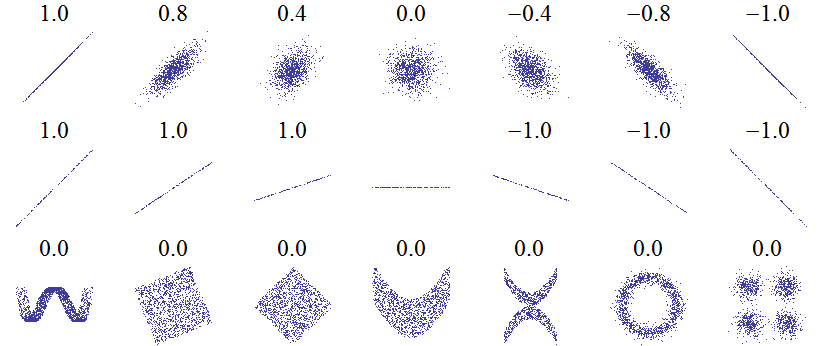
\includegraphics[scale=0.3]{rho_wiki}

\footnotesize
\href{https://commons.wikimedia.org/w/index.php?curid=15165296}{By DenisBoigelot, CC0} 
\end{center}

\end{frame} 


\begin{frame}{Correlation \& Independence}

If two RVs have $\rho=0$, that \textbf{tells us nothing} about whether they are independent.\\[1ex]

If two RVs are independent, their linear correlation ($\rho$) is zero, \textbf{and} their non-linear correlation (which we don't have a measure for\textcolor{magenta}{*}) is also zero.\\[1ex]

If you have not checked for nonlinear correlations, you have not checked if the RVs are independent.\\[1ex]

\footnotesize

\textcolor{magenta}{*There are several methods available for checking nonlinear correlations eg Spearman, Kendall.}
\end{frame} 


\section{Uncertainty Propagation}

\begin{frame}{Reminder of big picture}

\textbf{Measurements are meaningless without quoted uncertainties}. \\[1ex]

Very often, the thing we want to measure is not directly obtainable. It is a function of the RVs we measure, rather than the RVs themselves. \\[1ex]

How do we propagate the statistical uncertainties from the RVs to the function? \\[1ex]

\end{frame} 


\begin{frame}{LOTUS}
\footnotesize

A linear function \bbl{$f_1 = aX +b$} is a RV, so we calculate its expected value in the same way.\\[1ex]

Let's define our PDF for $X$ as $g_X$.\\[1ex]

$E[ X ] = \int x\, g_X\, dx $: expected value of RV $X$\\[1ex]

$E[ \bbl{f_1} ] = \int \bbl{f_1}\, g_f\, df = \int \bbl{f_1}\, g_X\,dx $: expected value of RV $\bbl{f_1}$\\[1ex]

This is known as LOTUS: The Law Of The Unconscious Statistician.\\[1ex]

Similarly, we can write the variance of a function: $V[ \bbl{f_1} ] = E[  ( \bbl{f_1} - E[ \bbl{f_1}) ] )^2 ]$.
\end{frame} 




\begin{frame}{A linear function of one variable}

$ \bbl{f_1 = aX +b}$ is a linear function of one RVs, and is itself a RV.\\

The \boo{Expected Value} of the function is:\\[1ex]
$E[\bbl{f_1} ] = E[ \bbl{aX + b} ] =  E[ aX] + E[ b ]  = \mathbf{a E[X] + b} $ \\

The \boo{Variance} of the function is:\\[1ex]
$V[\bbl{f_1} ] = V[ \bbl{aX + b}] =  \mathbf{a^2 V[X]}$  \textcolor{magenta}{*} \\

\tiny
\textcolor{magenta}{*proof:}\\
$E[\bbl{f_1}^2] =  E[ a^2X^2 + b^2 + 2abX ]  = a^2 E[X^2] +b^2 + 2ab E[X] $\\[1ex]
$E^2[\bbl{f_1}] =   a^2 E^2[X] + b^2 + 2abE[X]$\\[1ex]
$ V[\bbl{f_1} ] = E[\bbl{f_1}^2] - E^2[\bbl{f_1}] = a^2 E[X^2] +\cancel{b^2} + \cancel{2ab E[X]} - a^2 E^2[X] - \cancel{b^2} - \cancel{2abE[X]}$\\

\end{frame} 



\begin{frame}{A linear function of two variables}

$ \bbl{f_2 = aX + bY}$ is a linear function of two RVs, and is itself a RV.\\

%$ E[ \bbl{f_2}  ] =  \int\, \int \bbl{f_2} \, g_{XY}\, dx\, dy$   \\ 

The \boo{Expected Value} of the function is:\\[1ex]
$E[\bbl{f_2} ] = E[ \bbl{aX + bY} ] =   E[ aX] + E[bY ]  = \mathbf{a E[X] + b E[Y]}$ \\

The \boo{Variance} of the function is:\\[1ex]
$V[\bbl{f_2} ] = V[ \bbl{aX + bY}] = \mathbf{ a^2 V[X] + b^2 V[Y]  + 2ab\, \mathsf{cov}[X,Y]}$   \\
%= E[ ( aX + bY - E[ aX + bY ] )^2 ] \\
%= E[  ( aX -E[aX] + bY-E[bY] )^2  ]  \\
%= E[  ( aX -E[aX] )^2 + (bY-E[bY] )^2  + 2( aX -E[aX] ) ( bY -E[bY] )  ]\\
%= E[  ( aX -aE[X] )^2 + (bY-bE[Y] )^2  + 2( aX -aE[X] ) ( bY -bE[Y] )  ]\\
%= E[  a^2 V[X] + b^2 V[Y]  + 2ab cov[X,Y]  ]\\



\end{frame} 


\begin{frame}{A linear function of three variables}
\small

$\bbl{f_3 =  f(X,Y,Z) = aX + bY + cZ}$\\

\boo{Expected Value}: $E[ \bbl{f_3} ] = a E[X] + b E[Y] + cE[Z]$ \\

\boo{Variance}: $V[ \bbl{f_3} ] =  a^2 V[X] + b^2 V[Y]  + c^2 V[Z] + 2ab\, \mathsf{cov}[X,Y] + 2ac\, \mathsf{cov}[X,Z] + 2bc\, \mathsf{cov}[Y,Z] $   \\[2ex]

Tidied up: $V[ \bbl{f_3}  ]  = \sum\limits_{i=1}^{3} \sum\limits_{j=1}^{3} \alpha_i \alpha_j \mathsf{cov} [X_{(i)}, X_{(j)}]$\\[2ex]

When $i=j$ we get the terms like $a^2 V[X] $ because $cov[X,X] = V[X]$\\[1ex]
When $i\neq j$ we get the covariance terms (twice, for $i,j$ and $j,i$).\\[1ex]

\end{frame} 




\begin{frame}{A linear function of Z variables}

What we just did with $\bbl{f_3}$ can be extended to linear functions of any number of RVs.\\[1ex]

$\bbl{f_Z =\sum\limits_j^Z \alpha_j X_{(j)} }$\\

$E[ \bbl{f_Z} ] = E\left[ \bbl{\sum\limits_j^Z \alpha_j X_{(j)} } \right] =    \sum\limits_j^Z \alpha_j  E[ X_{(j)}] $ \blu{because E[sum] = sum(E)}\\[1ex]

$V[ \bbl{f_Z}  ] = \sum\limits_i^Z \sum\limits_j^Z \alpha_i  \alpha_j cov[X_{(i)} , X_{(j)}] $ \blu{as we demo'd on previous page.}\\[1ex]


\end{frame} 

\section{Taylor}
\begin{frame}{Taylor Series in a nutshell}
\footnotesize

\textbf{Consider a function}: $f(x) = \alpha_0 + \alpha_1 x +\alpha_2 x^2 + \alpha_3 x^3 + ....$\\[1ex]

When $x=0$, $f(x=0) = a_0$\\[1ex]
 
\blu{First derivative: $f'(x) = 0 +  \alpha_1 + 2 \alpha_2 x + 3 \alpha_3 x^2+ ... $}\\[1ex]
Evaluated at $x=0$: $f'(x=0) = \alpha_1$\\[2ex]

\blu{Second derivative: $f''(x) = 0 + 0+ 2 \alpha_2 + (3)(2) \alpha_3 x + ... $}\\[1ex]
Evaluated at $x=0$: $f''(x=0) = 2 \alpha_2$\\[2ex]

\blu{Third derivative: $f'''(x) = 0 + 0+ 0+ (3)(2) \alpha_3  + ... $}\\[1ex]
Evaluated at $x=0$: $f'''(x=0) = (3)(2) \alpha_3$\\[2ex]

And so on \textit{ad infinitum}.
\end{frame}


\begin{frame}{Taylor Series}
\footnotesize

$f(x) = \alpha_0 + \alpha_1 x +\alpha_2 x^2 + \alpha_3 x^3 + ....$\\[1ex]
$f(0) = a_0$\\[1ex]
$f'(0) = \alpha_1$\\[1ex]
$f''(0) = 2 \alpha_2$\\[1ex]
$f'''(0) = (3)(2) \alpha_3$\\[1ex]
The pattern gives us:\\[1ex]
$\alpha_n = \dfrac{f^n(0)}{n!}$ \blu{where $f^{n}$ means $n^{th}$ derivative of $f$}\\[1ex]
Which gives us the series: $f(x) = \sum\limits_{n=0}^\infty \dfrac{f^{\,n}(0)}{n!}   \,x^n $\\[1ex]
And generally, $f(x) = \sum\limits_{n=0}^\infty \dfrac{f^{\,n}(a)}{n!}   \,(x-a)^n $\\[1ex]

\boo{Notice that for a linear function of $x$, all terms after $n=1$ are zero.}

\end{frame}





\begin{frame}{$V[f_1]$ in terms of $V[X]$: Taylor expansion}
\footnotesize
We saw that we can write $V[\bbl{aX+b}] = a^2V[X]$ using algebra of expected values. Another option is to use the \textbf{Taylor expansion}, expanding the function about the expected value of the RV. We will use the notation $\mu \equiv E[x]$ and $f_{1}' \equiv \dfrac{df_1}{dx}$, so $f_{1\mu}' $ is the derivative of $f_1$ evaluated at $x=E[x]$\\[1ex]

\footnotesize
$\bbl{f_1} = \purp{f_{1\mu} } + \rbl{ f^{'}_{1\mu}}\, \gbl{(x - \mu) }$ \blu{linear in x, so two nonzero terms}\\[1ex]
$\left( \bbl{f_1} - \purp{f_{1\mu} } \right)^2 = \left( \rbl{f^{'}_{1\mu}}\, \gbl{(x - \mu) }\right)^2 $ \blu{square both sides}\\[1ex]

$E\left[( \bbl{f_1}- \purp{f_{1\mu} } )^2\right] = E\left[ \left( \rbl{ f^{'}_{1\mu} }\, \gbl{(x - \mu) } \right)^2 \right]$ \blu{expectation of both sides}\\[1ex]
$E\left[( \bbl{f_1}- \purp{f_{1\mu} } )^2\right]  =  \rbl{f^{'2}_{1\mu}} \, E[ \gbl{(x - \mu) } ^2 ] $ \blu{E[E[f]] = E[f]}\\[1ex]
$V[ f_1 ]  =  \rbl{f^{'2}_{1\mu}} \, V[X]\;\; \rightarrow\;\; V[ f_1 ]  =  \rbl{\dfrac{df_1}{dx}^2\bigg|_{x=\mu}}\, V[X]$\\[1ex]
\end{frame} 


\begin{frame}{$V[f_Z]$ in terms of $V[X]$: Taylor expansion}

We showed that $V[ f_1 ]  =  \dfrac{df_1}{dx}^2\bigg|_{x=\mu} V[X] $\\[1ex]

For a function of $Z$ RVs, $f_Z$, this becomes:\\

$V[ f_Z]  =  \displaystyle \sum\limits_i^Z \sum\limits_j^Z \blu{\dfrac{\partial f}{\partial x_{(i)} }  \dfrac{\partial f}{\partial x_{(j)} } \bigg|_{x_{(i,j)}=\mu}} \textcolor{magenta}{\mathsf{cov}[x_{(i)}, x_{(j)}]} =  \blu{\mathsf{J}}\, \covmat\, \blu{\mathsf{J^{T}}} $\\[1ex]

\blu{\textbf{J}} is the Jacobian matrix of partial derivatives, \blu{\textbf{J$^{\mathsf{T}}$}} is its transpose, and $\covmat$ is the covariance matrix.\\
\end{frame} 





\begin{frame}{Conclusion: Variance of a linear function}
\small
$
V[f_Z] = \blu{\mathsf{J}}\, \covmat\, \blu{\mathsf{J^{T}}} = 
\blu{\begin{bmatrix}
\dfrac{\partial {f_Z}}{\partial x_{(1)}}& ... & \dfrac{\partial {f_Z}}{\partial x_{(Z)}}
\end{bmatrix}}
\textcolor{magenta}{\begin{bmatrix}
\sigma^2_{x_{(1)}} & ... & \mathsf{cov}(x_{(Z)}, x_{(j)})\\
\vdots& \ddots & \vdots\\
\mathsf{cov}(x_{(i)}, x_{(Z)}) & ... & \sigma^2_{x_{(Z)}} \\
\end{bmatrix}
}
\blu{
\begin{bmatrix}
\dfrac{\partial {f_Z} }{\partial x_{(1)}}\\
 ... \\
 \dfrac{\partial {f_Z}}{\partial x_{(Z)}}
\end{bmatrix}
}
$
\vspace{0.5cm}

For a single function (not always the case, as we will see) and $Z$ RVs, the Jacobian matrix has 1 row and  $Z$ columns.\\[1ex]

Matrix multiplication rules tell us that $[1\times Z]\cdot[Z\times Z]\cdot [Z\times 1]= [1\times 1]$ : we have a single value for the variance as required.\\
\end{frame} 

\section{Nonlinear functions}

\begin{frame}
\centering
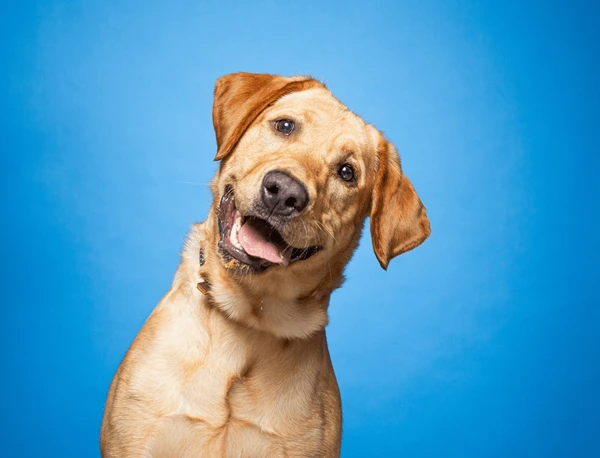
\includegraphics[scale=0.3]{doggo2}
\end{frame}


\begin{frame}{Covariance of nonlinear functions}
\footnotesize

We noted that we can write a linear function of $Z$ RVs as a sum: \\[1ex]

 $\bbl{f(X) =\sum\limits_j^Z \alpha_j X_{(j)} }$\\

A nonlinear function can be written as a product of linear functions: \\[1ex]

$\bbl{h(X) =\prod\limits_k^M\, f_k(X)}$\\

For example, $h(X)= aX^2 $ is a nonlinear function. We can write it as $h(X) = (aX)(X)$: the product of two linear functions $f_{k=1} = aX$ and $f_{k=2} = X$.\\[1ex]

\blu{In this simple example we have $M=2$ functions with $Z=1$ RV.}
\end{frame} 


\begin{frame}{Covariance of nonlinear functions}
\footnotesize

A product of $M$ functions means that we will have a [$M\times Z$] Jacobian Matrix \blu{\textbf{J}}.\\

For one function of $Z$ RVs: $
 \blu{\mathbf{J}}\, = 
\begin{bmatrix}
\dfrac{\partial {f}}{\partial x_{(1)}}& ... & \dfrac{\partial {f}}{\partial x_{(Z)}} \\
\end{bmatrix}
$
\vspace{0.5cm}

For two functions of $Z$ RVs: $
 \blu{\mathbf{J}}\, = 
\begin{bmatrix}
\dfrac{\partial {f_k}}{\partial x_{(1)}}& ... & \dfrac{\partial {f_k}}{\partial x_{(Z)}}\\[0.5ex]
\dfrac{\partial {f_l}}{\partial x_{(1)}}& ... & \dfrac{\partial {f_l}}{\partial x_{(Z)}} \\
\end{bmatrix}
$
\vspace{0.5cm}

For $M$ functions of $Z$ RVs: $
 \blu{\mathbf{J}}\, = 
\begin{bmatrix}
\dfrac{\partial {f_k}}{\partial x_{(1)}}& ... & \dfrac{\partial {f_k}}{\partial x_{(Z)}}\\
\vdots & \ddots & \vdots\\
\dfrac{\partial {f_M}}{\partial x_{(1)}}& ... & \dfrac{\partial {f_M}}{\partial x_{(Z)}} \\
\end{bmatrix}
$
\end{frame} 


\begin{frame}{Covariance of nonlinear functions}
\footnotesize

A product of $M$ functions means that we will have a [$M\times Z$] Jacobian, and instead of a single value for the variance we will have a [$M\times M$] matrix of values. Each element $V_{kl}$ of the matrix will be the variance for one of the linear functions.\\[2ex]

$V_{kl} =  \displaystyle \sum\limits_i^Z  \sum\limits_j^Z \blu{\dfrac{\partial f_k}{\partial x_{(i)}} \dfrac{\partial f_l}{\partial x_{(j)}}  \bigg|_{\mu}} \textcolor{magenta}{\mathsf{cov}[x_{(i)}, x_{(j)}]}$: \textbf{this is one of the $M^2$ variances}. \\[2ex]

The full $M\times M$ matrix of variances $V[h]$ can be written in the same simple way as before, but noting the Jacobian \blu{J} has changed shape:\\[1ex]
$V[h] =  \blu{\mathsf{J}}\, \covmat\, \blu{\mathsf{J^{T}}} $: this is a [$M\times M$] matrix of variances.\\[1ex]


\end{frame} 


\begin{frame}{Covariance of nonlinear functions}
\small

\textbf{What can we do with all this?}\\[1ex]

\footnotesize
\begin{itemize}
\item If we know the uncertainties (variance, covariance)\textcolor{magenta}{*} on our measurements, we can construct the covariance matrix, $\covmat$. 
\item If we know our functional form, we can construct the Jacobian, \blu{J}.
\end{itemize}
\vspace{0.5cm}

With these two ingredients, \textbf{we can calculate the uncertainty on our function}, as required. This is called  \textbf{propagation of uncertainties}.\\[1ex]

\blu{Note that we use the standard deviation $\sigma = \sqrt{V}$ for quoting uncertainties on a measurement (or on a function of measurements).}\\[1ex]

\textcolor{magenta}{*If all the RVs are independent, all the covariances are zero (nice and simple, but this is rarely true).}

\end{frame} 


\begin{frame}{Combining Systematic and Statistical Uncertainties}
\footnotesize
We can take into account systematic uncertainty by separating the measurement itself into a part with only systematic uncertainty and a part with only statistical uncertainty: $x = x_{a}+x_{b}$. \\[1ex]

The two parts are independent from one another, so the variance of the sum is the sum of the variances, and the uncertainties are added in quadrature:\\[1ex]

$V[x]  = V [x_a + x_b] =  V[x_a] + V[x_b]  =\sigma^2_{stat} + \sigma^2_{sys}$ \\

The covariance for two independent RVs with the same systematic uncertainty is simply $\sigma^2_{sys}$, as there is no statistical component of covariance between them (they are `statistically independent').\\[1ex]

$
\covmat = \begin{bmatrix}
\sigma^2_{stat} + \sigma^2_{sys} & \sigma^2_{sys}\\
\sigma^2_{sys} & \sigma^2_{stat} + \sigma^2_{sys} \\
\end{bmatrix}
$
\end{frame} 


\begin{frame}{Thanks For Your Time}
\center
\Huge
Fin.
\end{frame}






\end{document}

 
 